\section{Metodologia}

\subsection{Descrição do Sistema}
% Apresente os componentes do USV-Lab relevantes para a comunicação, como sensores, atuadores e infraestrutura de rede (baseada em mesh e VPN via 4G).
% Explique a integração com o framework MOOS-IvP.
O \textbf{VSNT-Lab} é um laboratório móvel da Marinha do Brasil integrado em uma embarcação de 7,7 metros (Flexboat SR 760), projetado para pesquisa e desenvolvimento de sistemas autônomos marítimos. Ele combina sensores avançados, atuadores e sistemas de controle baseados no framework MOOS-IvP para navegação e operações autônomas. O sistema inclui sensores como bússola GNSS, radar, sonar e câmeras PTZ, além de atuadores hidráulicos e motores potentes para controle de direção e velocidade.

\subsection*{Sistema de Comunicação}
O sistema de comunicação do VSNT-Lab, esquematizado na figura~\ref{fig:meto_vsntNetwork}, foi projetado para garantir conectividade confiável entre a embarcação e o navio-mãe. Ele utiliza uma configuração híbrida que combina:
\begin{itemize}
    \item \textbf{Rede Mesh}: Baseada no rádio NetNode para comunicação local de baixa latência.
    \item \textbf{Conexão 4G com VPN}: Para comunicação de longa distância, utilizndo o aplicativo TailScale para estabelecer uma VPN segura.
\end{itemize}

\begin{figure}[H]
    \caption{Sistema de Comunicação do VSNT-Lab}
       \centering
       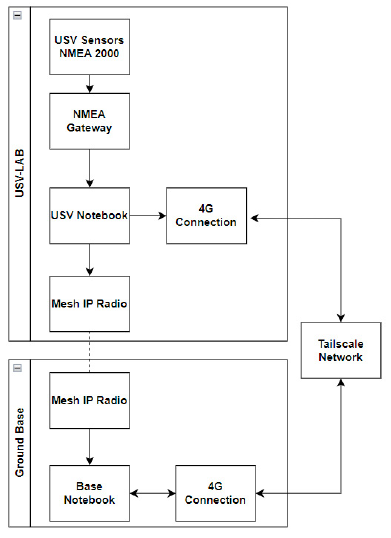
\includegraphics[height=8cm]{figuras/meto_vsntNetwork.png}
       \label{fig:meto_vsntNetwork}
   \small
   
   Fonte: Lima et al. \cite{VSNT_douglas2024}.
   \end{figure}

Essa infraestrutura é crucial para a operação remota e autônoma do sistema, permitindo controle, troca de dados e ajustes em tempo real.

\subsection{Coleta de Dados}
% Descreva os experimentos para coletar métricas de QoS (latência, perda de pacotes, jitter) durante missões simuladas e reais.
A coleta de dados para análise de comunicação entre o navio-mãe e o VSNT-Lab deve focar em métricas como latência, taxa de perda de pacotes, throughput e jitter. As medições devem ser realizadas em intervalos regulares, como a cada minuto, para gerar séries temporais detalhadas. Esses dados podem ser coletados tanto no canal mesh quanto na VPN e armazenados centralmente em um servidor, idealmente localizado no navio-mãe ou em uma base de apoio terrestre.

Para garantir a qualidade dos dados, é necessário filtrar medições afetadas por condições atípicas, como tráfego interno elevado, e descartar séries com número insuficiente de amostras. Um volume significativo de séries temporais, abrangendo diferentes condições operacionais, deve ser coletado para suportar análises robustas. Esse processo assegura que as medições reflitam fielmente o desempenho da rede em cenários operacionais reais.

\subsection{Modelagem com HMM}
% Utilize HMM para identificar estados ocultos de rede, como "rede boa", "rede degradada" e "rede indisponível".
Para modelar as condições da comunicação entre o navio-mãe e o VSNT-Lab, utilizaremos Cadeias de Markov Ocultas (HMM). O HMM é uma ferramenta poderosa para identificar padrões ocultos em séries temporais, como os estados subjacentes de uma rede de comunicação, a partir de observações visíveis, como métricas de desempenho. Neste contexto, definimos três estados ocultos principais: \textit{rede boa}, \textit{rede degradada} e \textit{rede indisponível}, cada um associado a probabilidades distintas de emissão das observações, como latência, taxa de perda de pacotes e jitter.

Cada estado oculto representa uma condição específica da rede. Por exemplo, o estado \textit{rede boa} está associado a baixas taxas de perda de pacotes e latências reduzidas, enquanto o estado \textit{rede degradada} reflete uma qualidade intermediária da comunicação, e o estado \textit{rede indisponível} caracteriza momentos de falha severa ou completa desconexão. A parametrização do modelo será realizada utilizando o algoritmo Baum-Welch, que ajusta as probabilidades de transição entre os estados ocultos e as probabilidades de emissão, com base nos dados coletados. Por meio do algoritmo de Viterbi, será possível inferir a sequência de estados ocultos mais provável a partir das métricas observadas, permitindo uma análise detalhada do desempenho da comunicação ao longo do tempo.

\subsection{Implementação de RL}
% Defina o MDP (estados, ações, recompensas) para gerenciar dinamicamente a troca entre os canais mesh e VPN.
A implementação de Aprendizado por Reforço (RL) será fundamentada no formalismo de Processos de Decisão de Markov (MDP), que modelam a dinâmica do sistema de comunicação do VSNT-Lab. O MDP será definido por um conjunto de estados (\textit{S}), representando as condições de rede detectadas pelo modelo HMM, um conjunto de ações (\textit{A}), que incluem a seleção do canal de comunicação (mesh ou VPN) ou ajustes nos parâmetros de transmissão, e uma função de recompensa (\textit{R}), projetada para incentivar decisões que maximizem a qualidade e estabilidade da comunicação.

Os estados (\textit{S}) incluirão informações sobre métricas observadas (como latência e perda de pacotes) e o canal atualmente ativo. As ações (\textit{A}) permitirão trocar dinamicamente entre os canais mesh e VPN ou manter a configuração atual. A função de recompensa (\textit{R}) será definida para penalizar mudanças desnecessárias de canal, latências elevadas e perdas de pacotes, enquanto valoriza ações que mantêm uma comunicação estável e eficiente. O algoritmo de Value Iteration será utilizado para encontrar a política ótima (\(\pi^*\)) que determina a melhor ação para cada estado, considerando um horizonte de planejamento e as restrições operacionais do sistema. Esta abordagem permitirá uma gestão inteligente e adaptativa da comunicação, reduzindo interrupções e otimizando o desempenho em cenários desafiadores.

\subsection{Validação}
% Teste o método em cenários reais, como operações militares e simulações na Baía de Guanabara e na Baía de Todos os Santos.
A validação do método proposto será realizada em cenários reais, explorando as operações de comunicação entre o navio-mãe e o VSNT-Lab. Os testes serão conduzidos em ambientes representativos, como a Baía de Guanabara e a Baía de Sepetiba, locais que oferecem desafios característicos de comunicação marítima, incluindo interferências ambientais, variações de distância e condições meteorológicas adversas.

Os experimentos incluirão a coleta de métricas de desempenho dos canais mesh e VPN em diferentes condições operacionais. Durante os testes, o modelo implementado será avaliado quanto à sua capacidade de identificar estados ocultos de rede, prever mudanças nas condições de comunicação e tomar decisões ótimas por meio do RL. As métricas de avaliação incluirão latência, taxa de perda de pacotes e a quantidade de mudanças de canal realizadas.

% \subsection{Ferramentas e Tecnologias}
% % Detalhe as tecnologias usadas, incluindo MOOS-IvP, infraestrutura de rádio mesh e VPN, e algoritmos de RL.